\chapter{Background}
\label{ch:Chapter2}
\section{Motivating example}
We use a DNN based Artificial Pancreas system(APS), closed-loop model, by Dutta et al. \cite{10.1007/978-3-319-99429-1_11}  as our motivating example for showing \attack. According to the APS, the patient relies on the model to predict the next dose of insulin to be injected into the body. 

%How is APS constructed?
The APS consists of sensors and an actuator, one that calculates the blood glucose values and one that injects the insulin inside the body respectively. The values from the two sensors are sent to the controller that calculates or predicts the next outcome. The network samples the previous blood glucose and insulin values discretized overtime at every 5 minutes. Such a model whose prediction depends on the data collected previously over time is called a data-driven model. The APS DNN model from Dutta et al. is shown in Figure 1. The DNN for APS is able to create mappings between the insulin and the glucose values that allow for the prediction of future insulin values. The model has 74 inputs in total as shown in Figure 1 where 32 inputs are the glucose and the rest are insulin values collected over a span of every 5 minutes. The DNN layers map these values with each other to predict the next value. 
\begin{figure}
	\centering
	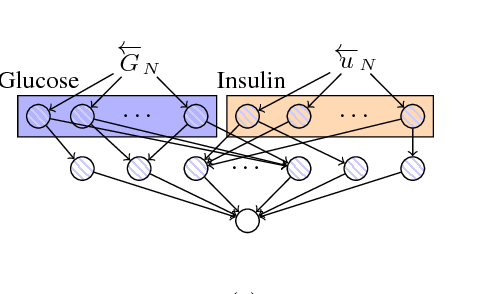
\includegraphics[width=0.7\linewidth, height=0.3\linewidth]{Images/APSDNN}
	\caption[APS DNN]{APS DNN designed by Dutta et. takes in 74 inputs of insulin and glucose. The next layers form connections between the insulin and the glucose to make predictions.}
	\label{fig:apsdnn}
\end{figure}

%Defense mechanisms
The APS DNN has certain defense mechanisms accompanying it. The DNN is accompanied by two DNNs that are trained to calculate the upper and the lower bounds to keep a check on the output prediction. In APS there is one output value that predicts the next outcome. Initially the expected output value is 140, after the attack the attacker changes it to 190. Due to the accompanying detection mechanisms, the attack will get detected. The range of acceptable output should be between 120-160. Hence, we want to perturb our inputs such that the output value is below 160 but much higher than 140. This is our motivation for designing an automatic attack synthesis mechanism. 

%This accompanying mechanism ensures that if the output value was supposed to be 140, does not change to 190 due to some malicious means. If the values don't lie within the bounds alarms are triggered. Our goal is to attack the system within these bounds and still cause some damage. 
%What is our goal
Since APS is a closed-loop system there is no human oversight. Consequently, it is important to ensure that the system is robust against ripples. We discuss our attack model in Section IV. 




%We use an Artificial Pancreas System(APS) as a running example to motivate the problem and illustrate our technique. This is an example of a safety-critical CPS that uses DNNs.\karthik{Please check}
%A patient using an APS relies completely on the closed-loop model of the APS\cite{10.1007/978-3-319-99429-1_11}. She trusts the model to monitor the body and deliver the right amount of insulin. %However, the APS does not consider side-channel attacks that can be conducted due to the CPS's interface and the presence of DNNs. \karthik{This should be in the Threat model section, not here}
%\karthik{Can you provide a brief description of the APS system, including the role of the DNN? - this is explained in the next paragraph}
%\karthik{You never talk about the DNN through}

%The attackers' goal is to change the inputs slightly such that the amount of insulin to be injected every time is more than the original amount that is supposed to be delivered.
%\karthik{What's the actual amount - the one that is supposed to be delivered when there is no attack}. 
%We want the inputs to be only minutely perturbed such that there is some output deviation observed from the original output. 

%There are two parts to conduct an attack. Since this is a data-driven attack \karthik{What's a data-driven attack? Either cite or define}, 
%the DNN predicts the output by taking in the inputs over time \karthik{What does over time mean?}. Hence, the network has 74 inputs in total \karthik{How does this follow?}. 
%Changing all 74 inputs is not feasible in a practical setting \karthik{What would it entail for the attacker to do this?}. 
%Hence, to conduct a successful ripple attack \karthik{We didn't say the attacker wants to conduct a ripple attack so far}, 
%the attacker needs to first find the critical input and perturb them by specific amounts \karthik{input or inputs}. 
%We provide a technique and automated tool for finding the critical input and further by finding the smallest possible perturbations to those inputs to cause a ripple.
%\karthik{Again, this is already explained in the intro - we need to be specific here} 

%Our proposed synthesized attack can ensure that the inputs are changed in a way that the output always lies within the upper and lower bounds set as constraints for the safety settings for the system. A consistent deviation from the actual value of insulin leads to damage to the patient.  \cite{ZHANG2019403}.

%\karthik{This section is very poorly written - please rewrite it}
%\aarti{Is it easy to understand this? - This is very important to highlight the importance of this work. - there are three models that are deployed together, hence we have to very carefully craft the attacks. }


\section{Problem Formulation}
%This section formulates the problem we are focusing on in this work. 
%We consider a closed-loop system as shown in Figure 2, with sensors as the inputs to the DNN and the actuators that take the output from the DNN based controllers. We describe the model for CPS, followed by the DNN controller model, attack model formalism and the problem statement.

%\aarti{Should the diagram be more descriptive with DNNs in the middle?}
\begin{figure}
	\centering
	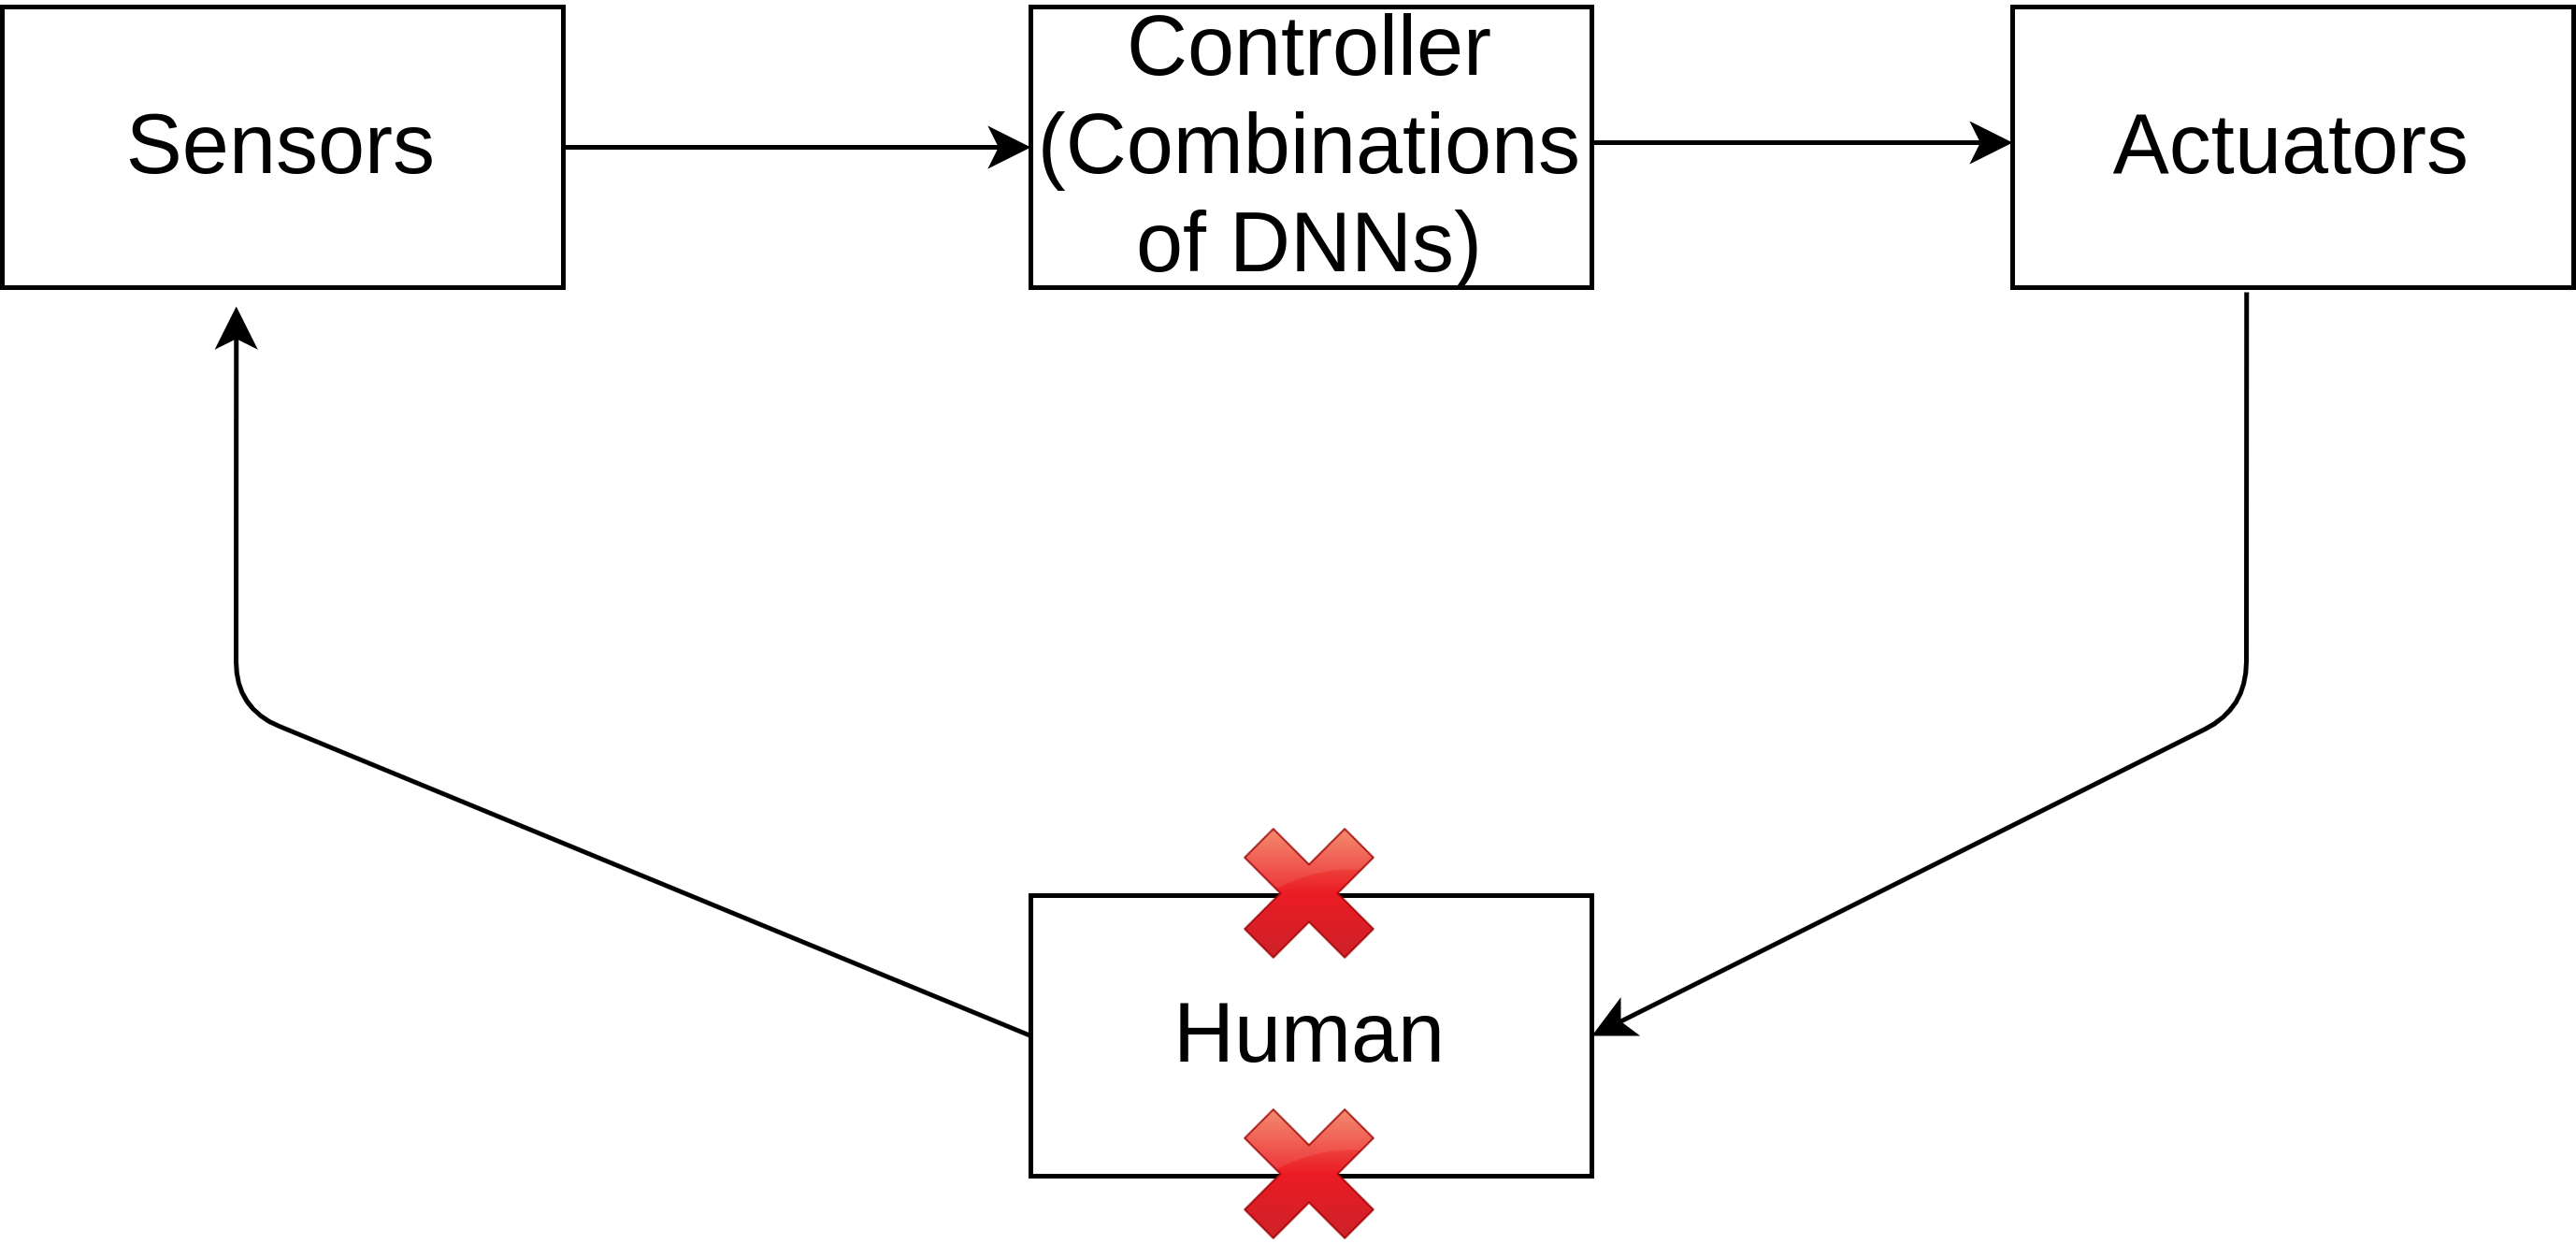
\includegraphics[width=0.7\linewidth]{Images/Systemsdescription}
	\caption[Closed-loop system]{General structure of a closed-loop system without the human involved in the process.}
	\label{fig:systemsdescription}
\end{figure}
\iffalse
\subsection{Controller for closed-loop system}
There are two types of CPS: open loop and closed loop. In open-loop systems, there is human intervention during the decision making process. In closed-loop systems, there are no regular human interventions as shown in Figure 2. In the latter cases understanding different types of security attacks becomes a necessity. In the case of stealthy (or subtle) attacks as described in the attack model section, the closed loops will not raise alarms. The reason is that the existing error-detection mechanisms are not aware of small perturbations from the original inputs under a constrained setting that can cause ripples. In DNN based CPS the decision making is accompanied by other DNNs that keep a track of the upper and the lower bounds for error-detection. 

%How does a controller work in a conventional setting
A conventional controller takes in the inputs collected through the sensors and processes the input for state estimation. There are multiple modes that are modeled inside the controller. Based on the inputs or the data collected from the sensors, the modes are selected. Every mode consists of a different set of equations.  The outputs are calculated based on the mode that then decides the next action to be taken by the system. 
\fi


\subsection{DNN Based Controller}
The conventional controller model is being replaced by DNN based controllers for CPS. One example is the DNN based controller designed by Dutta et al. \cite{Dutta_Others__2018__Robust}. Dutta et al. model robust DNN using the available patient data to predict the output in real-time as explained in Section III. Their controller design is for providing a data-driven approach for an artificial pancreas system (APS) which is also our first evaluation system.
\begin{figure}
	\centering
	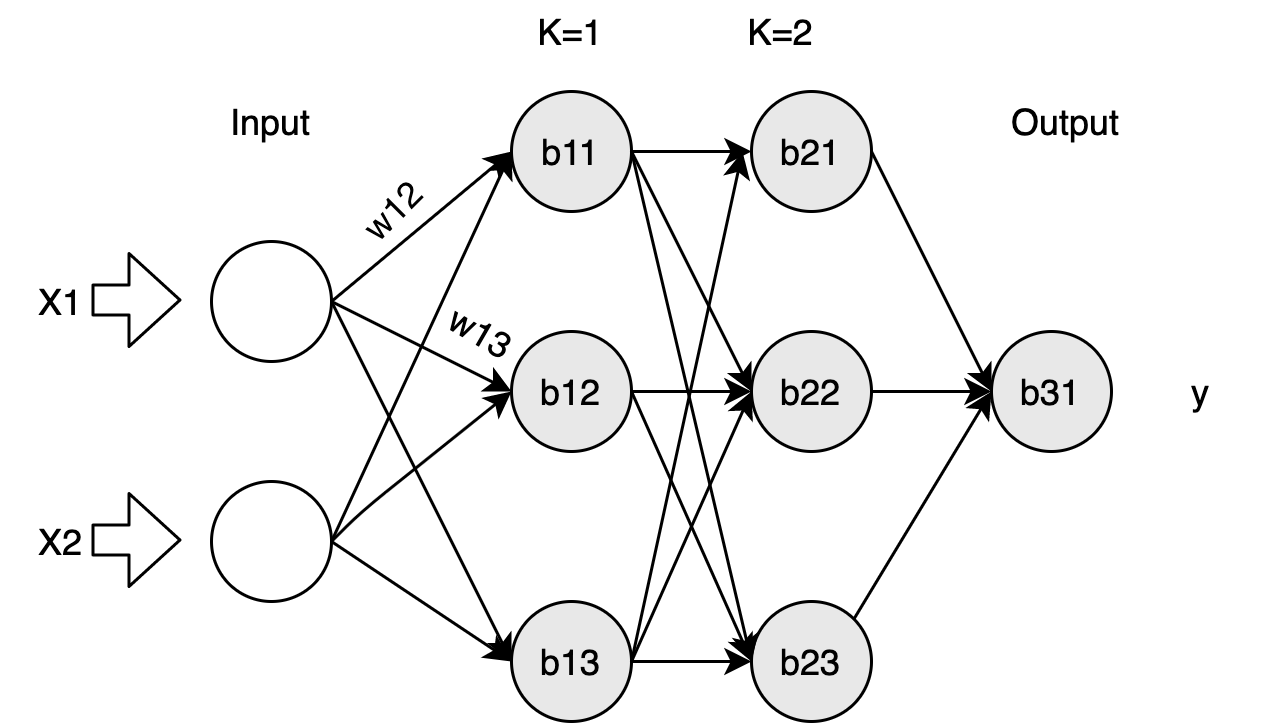
\includegraphics[width=0.7\linewidth]{Images/DNNstructure}
	\caption[DNN structure]{DNN controller structure with two hidden layers K=1,2, two inputs x1 and x2 and one output y. This is an example of a fully connected network.}
	\label{fig:dnn-controller}
\end{figure}

%Intro to the DNN structure
As mentioned in the previous sections, the controller is implemented by a DNN and not by conventional control theory. To explain the model in a simple way, we consider a feed-forward neural network with fully-connected layers. %The attack synthesis technique, however, will scale to other classes of DNNs such as recurrent DNNs or CNNs with some optimizations and modeling changes. 

%What does a DNN controller represent?
%What is a DNN made of?
The main purpose of a data-driven DNN based controller is that it maps the inputs that are the $x1$ and $x2$ to the output $y$ as per Figure 3. A DNN consists of multiple layers in the architecture that allows us to create the input-output mappings. The main components of the DNN are inputs, hidden layers, neurons in each hidden layer, the activation function applied to each layer in the network and the output. \textit{For our purposes to synthesize an attack we consider a trained neural network.} This means that all the components of the DNN are fixed.

%Formal modeling of a DNN for later use when explaining the modeling in MILP
The DNN consists of K layers numbered from 1 to K excluding the input layer.  The input layer can be numbered as K=0 and the final layer or the output is the K$^{th}$ layer.
The architecture can be represented as a function F defined as $F: X \rightarrow Y$ where the inputs X are mapped to the output Y and are composed of multiple layers. 

\begin{align*}
F(x) &= F_K \circ F_{K-1} \circ F_{K-2} ....... \circ F_1(x),    (1) \\
\end{align*}

$F_K$ represents the K$^{th}$ layer of the network. Each layer K$_{i}$, 
$i$ $\epsilon$ \{1,.,.,.,.,K\} consists of the smallest elements of a DNN called neurons as demonstrated in Figure 3.  Each neuron has a bias associated with it. Every neuron from the previous layer is connected to every neuron in the next layer. This is the property of a fully-connected network. 

Each output layer computes its output through the following formula. 
%\aarti{Check the consistency of symbols one more time. }

\begin{align*}
F_i(x) &= \upsigma(W_ix + b_i) ,  i = 1,.....,K, (2)  \\
\end{align*}

The $\upsigma$ is the abstraction for different activation functions that can be used to model the DNN as mentioned in the introduction. Our tool focuses on using Rectified Linear Unit (ReLU) since it is one of the most commonly used functions. %It is also piecewise linear so we can model it using MILP encoding. 

\begin{align*}
F_i(x) &= ReLU(W_ix + b_i) ,  i = 1,.....,K , (3) \\
\end{align*}

where, for a real vector x, ReLU(x):= max\{0,x\} (per layer).

During the training of the network, the parameters (weights and bias) are determined; we know those values when we are trying to find attacks on the CPS.

\subsection{Problem Statement}
%Given that we have the trained DNN model available, in the above section, we identify two problems that we are interested in solving. The first one is identifying the critical inputs in DNN based CPS and the second is synthesizing \attack with minimal cost. 

Given we have a trained DNN with fixed parameters our problem statement is to understand if the well-known FDI attacks in classical control theory are also valid in the DNN based CPS.
\begin{problem}
	How can we identify the critical inputs in a DNN?
\end{problem}

%Problem 2 is a follow up to the first problem. 

\begin{problem}
	What is the smallest perturbation to the critical input(s) that can result in ripple attacks in a limited time?
\end{problem}
%\smi{\attack is no longer in italics here, do we want to fix this? - interesting}

\begin{approach*}
	We abstract the DNN to a MILP problem to recognize the critical inputs to synthesize the \attack. We further model \attack specific cost functions to generate the new perturbed inputs for the attacks. 
\end{approach*}
